\documentclass{beamer}

\usepackage{amssymb}
\usepackage{amsfonts}
\usepackage{amsmath}
\usepackage{amsthm}
\usepackage{setspace}
\usepackage{longtable}
\usepackage{graphicx}
\usepackage{mathtools}
\usepackage{color}
\usepackage{array}
\usepackage{calc} 
\usepackage{bm}
\usepackage{caption}
\usepackage{float}

\usetheme{CambridgeUS}
\useoutertheme{infolines}
%numbering
\setbeamercolor{background canvas}{bg=white}
\setbeamersize{text margin left=1cm,text margin right=1cm}

\title[AI1110  Assignment-6]{ASSIGNMENT-6}
\subtitle{AI1110}
\author[]{MUKUNDA REDDY \\ AI21BTECH11021}
\date{}

\begin{document}
  \begin{frame}
      \titlepage
  \end{frame}
  
  \begin{frame}{Outline}
      \tableofcontents
  \end{frame}
  
  \section{Question}
  \begin{frame}{Example:6-4}
  Find the probaility mass distribution of two random variables for each of the following? \\
  \begin{enumerate}[a]
      \item In the fair-die experiment random variable
            $x(f_i)$ equals the number of dots shown and y
            equals twice this number. \\
      \item Toss the die twice  and  define random variables 
            x and y such that x equals the first number that 
            shows, and y shows second. \\
      \item  The die is tossed twice such that 
              $$ x(f_i f_k)=|i-k| ,\: y(f_i f_k)=i+k$$.\\
  \end{enumerate}
  \end{frame}
  
  \section{Solution}
  \subsection{EX:6-4 (a)}
  \begin{frame}{Example:6-4 (a) Solution}
   Given $x(f_i)=i$ and $y(f_i) = 2i$ for $i=1,2,...6$ \\
   in other words $x_i = i , y_k = 2i$ and
   \begin{center}
   \[
      p_{ik} = P\{ x=i,y=2k \} =
   \begin{cases}
   \frac{1}{6} & i=k \\
     0   & i \neq k \\
   \end{cases}
   \]
    \end{center} 
    Thus there are masses only on six points $(i,2i)$ and mass of each point equals $\frac{1}{6}$.\\
  \end{frame}
  
  \begin{frame}{Example:6-4 (a) Solution}
  \begin{figure}
      \centering
      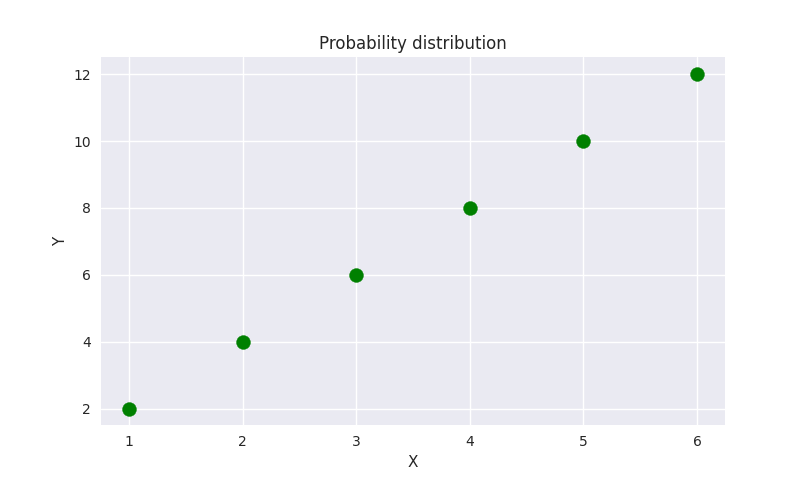
\includegraphics[scale=0.5]{Figure_1.png}
      \caption{6-4 (a)}
      \label{fig:(a)}
  \end{figure}
      
  \end{frame}
  
  \subsection{EX:6-4 (b)}
  \begin{frame}{Example:6-4 (b) Solution}
      We toss the dice twice so we get 36 outcomes $f_i f_k$. \\
      
      Let random variables is defined as 
      $$ x(f_i f_k)=i,\:y(f_i f_k)=k\:\:\:\{i,k=1,2....6\} $$ \\
      
      Thus $x_i = i,y_k =k,$ and $p_{ik} = \frac{1}{36}$.We therefore have 36 point masses and the mass of each point equals $\frac{1}{36}$.On the line $x = i$ there are 6 points with total mass $\frac{1}{6}.$
  \end{frame}
  
  \begin{frame}{Example:6-4 (b) Solution}
      \begin{figure}
          \centering
          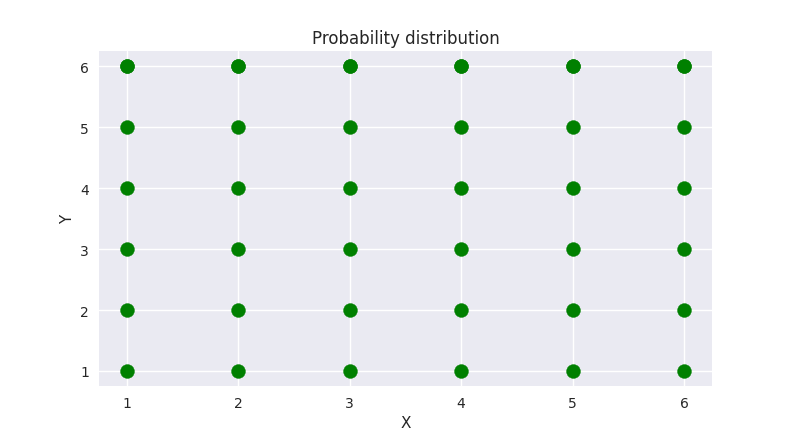
\includegraphics[scale=0.5]{Figure_2.png}
          \caption{6-4 (b)}
          \label{fig:(b)}
      \end{figure}
  \end{frame}
  
  \subsection{EX:6-4 (c)}
  \begin{frame}{Example:6-4 (c) Solution}
  We toss die twice In this case $x$ takes $0,1,2,...5$ and
  $y$ takes the values $2,3,...12$.This gives $6 \times 11 = 66 $ but only 21 positive mass points are found.\\
  \begin{center}
  $$ x(f_i f_k)=|i-k| ,\: y(f_i f_k)=i+k$$.\\
  \end{center}
  Consider the case $x=0$  then $y= 2,4,..12$.if $x=0$,then
  $i=k$ and $y=2i$.There are 6 mass points in the line and mass
  of each point equals $\frac{1}{36}$.
  \end{frame}
  
  \begin{frame}{Example:6-4 (c) Solution}
  If $x=1$,then $y=3,5,...11$.Thus,there are,five mass points
  on the line $x=1$ and mass of each point equals
  $\frac{2}{36}$. \\
  
  Consider $x=1$ and $y=7$ then there are two posibilities
  they are $i=3,k=4$ and $i=4,k=3$. \\
  $$\text{Hence  } P\{x=1,y=7\} = \frac{2}{36}$$. \\
  
  From the figure \ref{fig:(c)} all those that are circles has 
  masses $\frac{2}{36}$ and triangles has masses $\frac{1}{36}$
  
  
      
  \end{frame}
  
  \begin{frame}{Example:6-4 (c) Solution}
      \begin{figure}
          \centering
          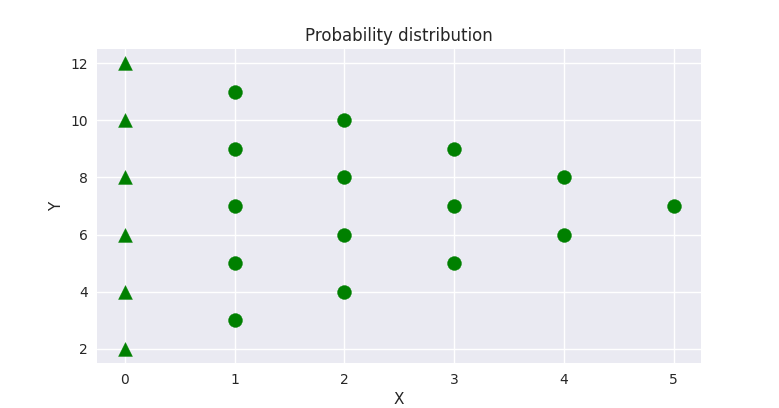
\includegraphics[scale=0.5]{Figure_3.png}
          \caption{6-4 (c)}
          \label{fig:(c)}
      \end{figure}
  \end{frame}

\end{document}